\clearpage\null\vfill
\thispagestyle{empty}
\begin{minipage}[b]{.9\textwidth}
  \begin{center}
  \setlength{\parskip}{.5\baselineskip}
  {\color{phdcol0}%
   \ccLogo\hspace{.1cm}%
   \ccAttribution\hspace{.1cm}%
   \ccNonCommercial\hspace{.1cm}%
   \ccNoDerivatives}\hspace{.15cm}%
  \footnotesize%
  This work is licensed under {\color{phdcol1}\textbf{http://creativecommons.org/licenses/by-nc-nd/3.0/}}
  \end{center}
\end{minipage}
\vspace*{2\baselineskip}
\clearpage
\thispagestyle{empty}
\vspace*{\stretch{1}}
\begin{flushright}
  \textit{À Seref, Keziban, Didem et Ilayda.}
\end{flushright}
\vspace*{\stretch{7}}
%
%%
%\chapter*{Remerciements}
%
%
%\`A tous, \textbf{merci infiniment} !
%

\chapter*{Résumé Long}


Cette thèse traite la résolution du problème de satisfaisabilité booléenne (SAT).
SAT permet de résoudre des problèmes importants dans différents domaines tels 
que la planification~\cite{planning_92}, la biologie~\cite{biology_06}, la vérification de logiciel et de 
matériel~\cite{biere1999symbolic}, de raisonnement automatique~\cite{heule2016solving}, etc.
Leurs évolutions au cours des dernières décennies leur ont permis de traiter des problèmes de plus en plus complexes.
Des travaux récents ont réussi a prouver à l'aide d'un solveur SAT, une borne maximum
pour le problème de coloration des triplets pythagoriciens, avec une preuve de 200 TB~\cite{heule2016solving}.


Étant donné un problème SAT, l'objectif est de  déterminer si il est possible de satisfaire toutes les contraintes du
problème, si c'est le cas on dit que le problème est satisfaisable, sinon il est insatifaisable.
% satisfaisable ou non.
%
% c'est à dire que toutes les contraintes peuvent être satisfaites,
%ou insatisfaisable, c'est-à-dire qu'il n'y a aucun moyen de satisfaire toutes les contraintes avec une même affectation.
Ce calcul est effectué par un solveur SAT qui répond $\sat$ lorsque la formule est satisfaisable et $\unsat$ dans le cas
contraire. SAT a été le premier problème ayant été prouvé NP-Complet~\cite{cook1971complexity}. Cela signifie que
l'on ne connait pas d'algorithme capable de résoudre le problème avec une complexité polynomiale.
%La résolution du problème est l'un des sept prix du millénaire, à savoir P = NP.


Malgré cette complexité, les solveurs SAT sont capables de résoudre de plus en plus de problèmes complexes.
Ce succès vient de l'introduction de différentes heuristiques sophistiquées et de 
l'algorithme de résolution utilisé, $\guillemotleft$ Conflict Driven Clause Learning$\guillemotright$ (CDCL).
Il est basé sur l'algorithme DPLL nommé suivant ses auteurs Davis, Putnam, Logemann et Loveland~\cite{dpll_62},
l'un des premiers algorithmes avec une utilisation non intensive de la mémoire.

%
%Cet algorithme est basé sur  
%et Loveland (DPLL)\cite{dpll_62}.
%
%
%l'optimisation de l'algorithme de
%résolution des conflits appelé $\guillemotleft$ Conflict Driven Clause Learning$\guillemotright$ (CDCL) qui est basée sur le premier
%algorithme (avec une utilisation non intensive de la  mémoire) nommé par ses auteurs Davis, Putnam, Logemann
%et Loveland (DPLL)\cite{dpll_62}.

Le CDCL peut être vu suivant l'exploration d'un arbre binaire avec au total $2^n$ branches, avec $n$ le nombre de variables du problème.
La première étape consiste à choisir une variable dite de décision, puis d'effectuer les déductions logiques à partir de l'affection. 
Si l'algorithme se trouve dans une situation de conflit, c'est-à-dire que l'affectation courante n'est pas capable de satisfaire au moins une contrainte du problème, l'algorithme  calcule une clause dite de conflit qui permet d'élaguer 
cet espace de recherche. Avec cette contrainte le solveur effectue un \textit{backjump}, c'est-à-dire qu'il remonte dans l'arbre
de recherche pour explorer une autre branche.
%Cette clause est une information redondante par rapport au problème initial.
Si aucun conflit n'est présent, l'algorithme choisit à nouveau une variable de décision. L'algorithme termine  soit lorsque toutes les variables sont affectées auquel cas le problème est satisfaisable, soit lorsque un conflit est apparu avec uniquement des déductions logiques auquel cas le
problème est non satisfaisable.
La Figure~\ref{fig:cdclflow} présente sous forme d'un organigramme le fonctionnement de l'algorithme CDCL.

\begin{figure}[!htbp]
\begin{tikzpicture}[node distance=1.5cm,
,every node/.style={scale=0.7,fill=white, font=\sffamily}, align=center]
% Specification of nodes (position, etc.)
\tikzset{%	
	>={Latex[width=2mm,length=2mm]},
	% Specifications for style of nodes:
	base/.style = {rectangle, rounded corners, draw=black,
		minimum width=2cm, minimum height=1cm,
		text centered, font=\sffamily},
	question/.style = {base, diamond, fill=blue!15},
	unsat/.style = {base, fill=red!30,minimum width=3cm},
	sat/.style = {base, fill=green!30,minimum width=3cm},
	process/.style = {base, minimum width=2.5cm, fill=orange!15,
		font=\ttfamily},
}
\node (isfin) [question] {Variables toutes \\assignées ?};
\node (dec)     [process, below = of isfin]          {Choix variable \\ de decision};
\node (sdec)     [right = of dec]          {};
\node (idec) [left = of isfin]  {};
\node (prop)    [process, below = of dec ]          {Propagation unitaire};
\node (conf)    [question, below = of prop] { Conflit ?};
\node (confanalyse) [process, below = of conf] {Analyse du \\ conflit};
\node (learn) [process] at ($(prop) + (160pt, 0)$) {Apprentissage de la \\ clause de conflit};
\node (isend) [question] at ($(confanalyse) + (160pt, 0)$) {Niveau de \\decision zero ?};
\node (end) [unsat] at ($(isend) + (140pt, 0)$) {$\unsat$};
\node (ends) [sat] at ($(isfin) + (+160pt, 0)$){$\sat$};


\draw[->, thick]     (sdec) -- (dec);
\draw[->, thick]     (dec) -- (prop);
\draw[->, thick]     (prop) -- (conf);
\draw[->, thick]     (conf) -| node [yshift=5.5 cm] {non}(idec.center) -- (isfin);
\draw[->, thick]     (conf) -- node {oui} (confanalyse);
\draw[->, thick]     (isfin) -- node {non}(dec);
\draw[->, thick]     (confanalyse) --(isend);
\draw[->, thick]     (isend) -- node {oui}(end);
\draw[->, thick]     (isfin) -- node {oui}(ends);
\draw[->, thick]     (learn) -- (prop);
\draw[->, thick]     (isend) -- node [] {non}(learn);

\end{tikzpicture}
\caption{Organigramme de l'algorithme CDCL}
\label{fig:cdclflow}
\end{figure}

%\begin{figure}[!htbp]
%	\begin{tikzpicture}[node distance=1.5cm,
%	,every node/.style={scale=0.7,fill=white, font=\sffamily}, align=center]
%	% Specification of nodes (position, etc.)
%	\tikzset{%	
%		>={Latex[width=2mm,length=2mm]},
%		% Specifications for style of nodes:
%		base/.style = {rectangle, rounded corners, draw=black,
%			minimum width=2cm, minimum height=1cm,
%			text centered, font=\sffamily},
%		question/.style = {base, diamond, fill=blue!15},
%		unsat/.style = {base, fill=red!30,minimum width=3cm},
%		sat/.style = {base, fill=green!30,minimum width=3cm},
%		process/.style = {base, minimum width=2.5cm, fill=orange!15,
%			font=\ttfamily},
%	}
%	\node (isfin) [question] {All vars\\ assign?};
%	\node (dec)     [process, below = of isfin]          {Choose decision var};
%	\node (sdec)     [right = of dec]          {};
%	\node (idec) [left = of isfin]  {};
%	\node (prop)    [process, below = of dec ]          {Unit Propagation};
%	\node (conf)    [question, below = of prop] { IsConflict?};
%	\node (confanalyse) [process, below = of conf] {Conflict Analysis};
%	\node (learn) [process] at ($(prop) + (160pt, 0)$) {Learn conflict clause};
%	\node (isend) [question] at ($(confanalyse) + (160pt, 0)$) {is level\\zero?};
%	\node (end) [unsat] at ($(isend) + (140pt, 0)$) {$\unsat$};
%	\node (ends) [sat] at ($(isfin) + (+160pt, 0)$){$\sat$};
%	
%	
%	\draw[->, thick]     (sdec) -- (dec);
%	\draw[->, thick]     (dec) -- (prop);
%	\draw[->, thick]     (prop) -- (conf);
%	\draw[->, thick]     (conf) -| node [yshift=5.5 cm] {no}(idec.center) -- (isfin);
%	\draw[->, thick]     (conf) -- node {yes} (confanalyse);
%	\draw[->, thick]     (isfin) -- node {no}(dec);
%	\draw[->, thick]     (confanalyse) --(isend);
%	\draw[->, thick]     (isend) -- node {yes}(end);
%	\draw[->, thick]     (isfin) -- node {yes}(ends);
%	\draw[->, thick]     (learn) -- (prop);
%	\draw[->, thick]     (isend) -- node [] {no}(learn);
%	
%	\end{tikzpicture}
%	\caption{Organigramme de l'algorithme CDCL}
%	\label{fig:cdclflow}
%\end{figure}


Certains problèmes présentent des symétries, dans ce cas, des branches de l'espace de recherche 
sont identiques à une permutation près, on dit que cet espace de recherche est isomorphe.
Si une branche de l'espace de recherche est solution du problème alors toutes les branches symétriques
sont également des solutions. Dans le cas inverse si il n'existe pas de solution dans une branche alors il n'en
existe dans aucune des branches symétriques.
En parcourant les espaces isomorphes, le solveur effectue donc du travail inutile.

Pour illustrer ce problème, prenons comme exemple le problème des tiroirs (\textit{pigeonhole problem}) dans lequel nous avons un ensemble de pigeons qui doivent êtres attribués à des nids différents. Dans ce problème il y a un nid de moins que le nombre de pigeons.
Le but de ce problème est de déterminer s'il est possible d'attribuer un nid différent à chaque pigeon.
La figure~\ref{fig:holefr} présente une instance de ce problème.


\begin{figure}[!htbp]
	\centering
	\begin{tikzpicture}[
	start chain = going right,
	node distance = 0pt,
	AStyle/.style={draw, minimum width=2em, minimum height=2em, 
		outer sep=0pt, on chain, fill=yellow!0!white}]
	\node [AStyle] (1) {\huge\textcolor{gray}{\PHdove}};
	\node [AStyle] (4) {\huge\textcolor{gray}{\PHdove}};
	\node [AStyle] (5) {\huge\textcolor{gray}{\PHdove}};
	\node [AStyle, draw] (6) {\huge\textcolor{gray}{\PHdove}};
	\node [ minimum width=2em, minimum height=2em, 
	outer sep=1pt, on chain] (7) {\huge\textcolor{gray}{\PHdove}};
	\end{tikzpicture}
	\caption{Représentation graphique d'une instance du problème des pigeons (5 pigeons, 4 nids)}
	\label{fig:holefr}
\end{figure}


Pour un humain, la réponse à ce problème est évidente, mais un solveur de l'état de l'art va parcourir toutes 
les combinaisons possibles de couples (pigeon, nid) et cela le mène à une explosion combinatoire.
Pour cette raison, résoudre ce problème avec un solveur SAT standard s'avère très chronophage et même impossible dans des temps raisonnables
pour un nombre de pigeons supérieur à 15.

%Cependant, certains problèmes possèdent un espace de recherche énorme et ne peuvent pas 
%être traité par un solveur SAT. Un exemple d'un tel problème peut être le problème de tournées de véhicules (VRP). 
%Il s'agit du service d'entreprise de livraison, dans lequel étant donné une flotte de véhicules basés dans un dépôt, ceux ci doivent faire des rondes entre des clients qui ont demandés chacun une certaine quantité de marchandises. Le circuit effectué par un véhicule pour la visite de tous les clients
%est appelé la tournée du véhicule. L'objectif est de trouver la tournée qui minimise les coûts de livraison (monétaire, distance, temps, ....).
%
%
%Dans le problème précédent, renommer l'ensemble de véhicules identiques nous donnera exactement le même problème. C'est ce qu'on appelle une symétrie.

De manière plus  générale, une symétrie est une transformation qui laisse un objet (ou un aspect de l'objet) inchangé. Les symétries sont généralement définies comme une propriété syntaxique d'un problème lorsque leur présence est inhérente à l'encodage du problème.
Dans ce cas, une permutation des variables préserve la spécification originale du problème.
Dans le cas où les symétries sont indépendantes d'une représentation particulière du problème, il s'agit de symétries sémantiques.

La présence de symétrie dans un problème force l'algorithme de recherche à explorer en vain l'espace de recherche symétrique et impacte considérablement ses performances.  La rupture de symétrie est une approche qui évite au solveur de visiter les espaces de recherche isomorphes.

Pour pouvoir exploiter les symétries, la première étape consiste à les trouver. Dans le contexte de la satisfaction booléenne, la détection des symétries syntaxiques se fait tout d'abord par la transformation de la spécification en un graphe coloré et ensuite par l'application d'un outil d'automorphisme de graphe sur celui-ci.
Différents outils traitent de ce problème dans l'état de l'art, tels que, $\bliss$~\cite{JunttilaKaski:ALENEX2007}, $\saucy$~\cite{katebi2010symmetry}, …


Lorsque les symétries sont obtenues, la façon la plus courante pour les exploiter est d'utiliser une approche de rupture de symétrie statique. Elle est dite statique, car le traitement de cette approche  est effectuée avant la résolution du problème SAT.
Ceci consiste à prendre le problème symétrique en entrée et à produire une formule à satisfaction équivalente, en éliminant les symétries présentes. %Le problème en sortie ne peut pas être insatisfaisable si le problème initial est satisfaisable.
Pour produire une formule équivalente sans présence de symétries, le problème est augmenté par des 
contraintes de rupture de  symétries  (\textit{symmetry breaking predicates sbp)}.
 Celles-ci empêchent le solveur d'explorer les espaces de recherche isomorphes. 
Si l'on considère l'exemple précédent avec les pigeons, le premier pigeon est attribué a un
exactement un nid, la symétrie est alors «rompue».

Plusieurs outils, tels que $\shatter$~\cite{aloul06} et $\breakid$~\cite{devriendt2016improved}, utilisent cette technique pour accélérer le calcul du solveur en présence de symétries.
En général, cette approche aboutit à de bons résultats dans différentes instances symétriques, cependant elle possède des défauts. Parmi eux, nous pouvons citer le nombre de contraintes ajoutées qui peut être exponentiel par rapport à la taille du problème. Ceci 
a pour conséquence de ralentir l'algorithme principal du solveur.
De plus, étant donné que ce calcul est effectué avant le lancement du solveur, cette approche peut être difficilement combinée avec d'autres techniques de rupture de symétries. Aussi, cette approche ne peut pas distinguer les contraintes originales du problème avec les contraintes de rupture de symétrie. Avec cette information, le solveur peut modifier ses heuristiques pour augmenter ses performances.
Pour ces raisons, certains problèmes avec de nombreuses symétries ne peuvent pas être traités efficacement avec cette approche.

Une autre approche dite rupture de symétrie dynamique consiste à utiliser les symétries durant l'algorithme de recherche du solveur SAT, plus précisément, à modifier son comportement pour exploiter les propriétés de symétrie du problème. Cette approche consiste à déduire des faits symétriques par rapport aux déductions effectuées par le solveur. Lorsque ces faits sont ignorés, le solveur va explorer en vain l'espace de recherche symétrique.
Ces déductions réduisent le nombre de décisions, qui sont des suppositions du solveur choisies de 
manière heuristique, et augmentent le nombre de propagations qui sont les déductions logiques faites par le solveur. 
Cette approche transforme donc les suppositions du solveur en déductions logiques.
Différents outils utilisent cette approche, nous pouvons citer \textit{Symmchaff}
qui n'exploite que certains types spécifiques de symétries, \textit{Symmetry Propagation (SP)}, \textit{Symmetry Learning Scheme (SLS)} et \textit{Symmetry Explanation Learning (SEL)} qui ajoutent les symétriques des
clauses apprises pour permettre les déductions symétriques.
Étant donné que cette approche est dynamique, il est possible pour le solveur 
d'intégrer des heuristiques spécifiques ou encore de combiner les différentes techniques de rupture de symétrie.


Cette thèse vise à améliorer l'existant et rendre les solveurs plus performants en présence de symétries et
propose différentes contributions allant dans ce sens.  


Notre première contribution mime le comportement de la rupture de symétrie statique, mais 
opère dynamiquement, pendant l'exécution du solveur. On ajoute dans le solveur un composant de symétrie opportuniste qui va détecter que le solveur parcourt un espace de recherche symétrique et va ajouter à celui-ci une contrainte appelée $\guillemotleft$ effectective symmetry breaking predicate $\guillemotright$ qui va empêcher le solveur de rester dans
l'espace de recherche en question. Cela a pour conséquence de réduire le nombre de contraintes et donc 
ne ralentit pas le solveur.

% Cette contrainte est dite effective, car 
% à l'inverse de l'approche 
%de rupture de symétrie  statique la contrainte est forcément utilisée par le solveur. Aucune contrainte
%inutile n’est insérée dans le solveur. 

Ce composant de symétrie est fourni sous forme d'une bibliothèque codée en C++ et se nomme $\libdsb$.
Elle peut s'interfacer avec n'importe quelle solveur de type CDCL. 
Pour conduire nos expériences, nous l'avons interfacée avec un solveur de l'état de l'art nommé $\minisat$~\cite{een2003extensible}. Au total, l'intégration de $\libdsb$ ajoute environ 60 lignes de code 
et augmente le code de $\minisat$ de 3\%.
$\libdsb$ est $\guillemotleft$ open source $\guillemotright$, fourni sous une licence GPLv3 et est disponible sur Github \footnote{\url{https://github.com/lip6/cosy}}.


Pour évaluer notre approche, nous avons comparé une version du solveur $\minisat$ combiné avec la bibliothèque $\libdsb$, que nous avons appelé $\cdclsym$ avec les solveurs de l'état de l'art.
Ces expérimentations ont été effectuées sur les instances de la SAT Competiton~\cite{jarvisalo2012international} sur les dernières années (2012 - 2017) pour lesquelles $\bliss$ a réussi a trouver des symétries. Au total, nous avons obtenu 1350 instances.

La figure~\ref{fig:frcactus} nous montre les résultats obtenus sous forme d'un cactus plot, 
dans lequel l'axe des abscisses nous montre le nombre d'instances réussies par chacun des solveurs et l'axe des ordonnées nous montre le temps de calcul des solveurs.
Nous avons conduit ces expériences avec deux outils d'automorphisme de graphe, à savoir 
$\saucy$ à gauche de la figure et $\bliss$ à droite de la figure. 

Comme nous pouvons le constater, les résultats sont meilleurs  avec l'utilisation de l'outil d'automorphisme de 
graphe $\bliss$. La principale différence entre les deux outils est le nombre de permutations obtenues.
$\bliss$ nous donne plus de permutations que $\saucy$, cela permet a notre outil $\cdclsym$ d'atteindre 
un nombre d'instances résolues de 775 alors que le deuxième meilleur outil $\breakid$ atteint un nombre d'instances résolues de 749 avec $\bliss$. Toutes les expériences étaient limitées à une durée à 5000 secondes.

Ces expériences nous démontrent que notre approche est aussi performante que les approches de rupture de symétrie statique.
\begin{figure}[!htbp]
	\centering
	\subfloat[avec \saucy]{{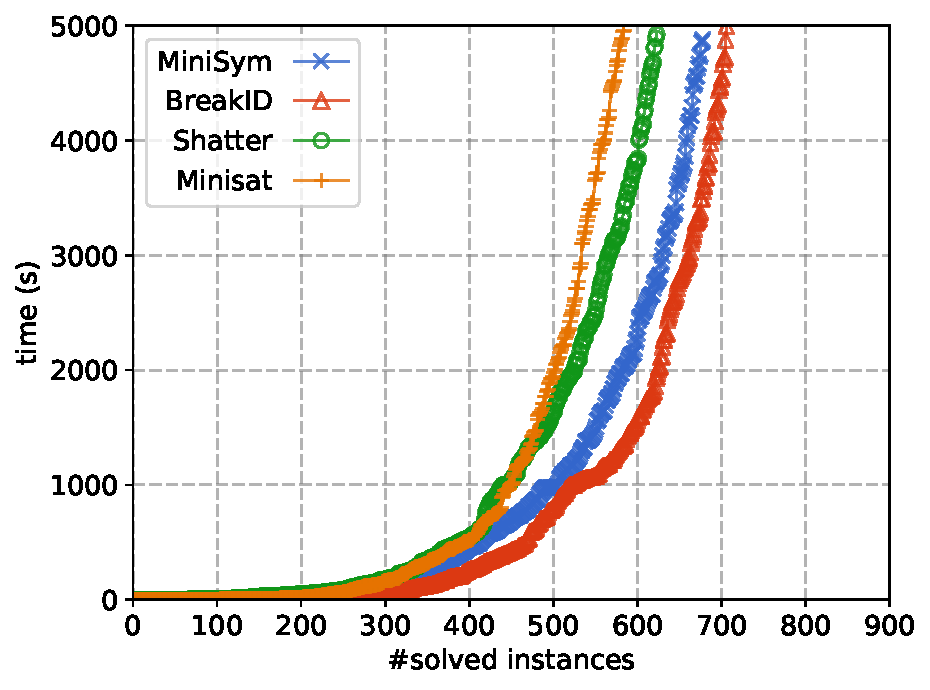
\includegraphics[scale=0.36]{img/saucy-result}}}%
	\qquad
	\subfloat[with \bliss]{{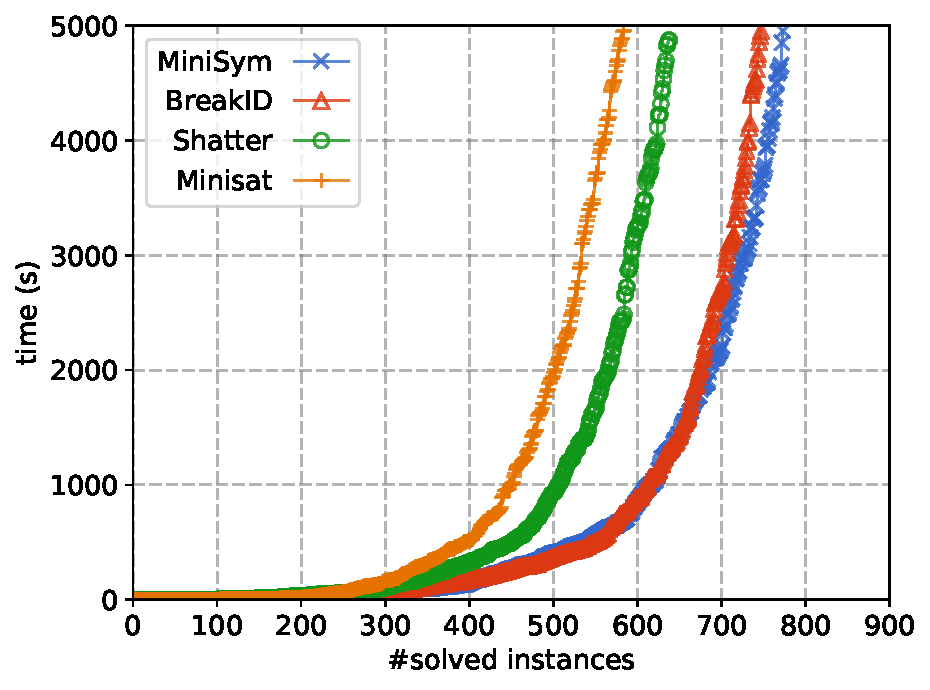
\includegraphics[scale=0.36]{img/bliss-result}}}%
	\caption{Cactus plot  présentant le nombre total d'intances résolues}%
	\label{fig:frcactus}%
\end{figure}

Malgré les très bons résultats obtenus par notre approche, certains problèmes qui sont résolus très 
rapidement par les approches de rupture de symétrie dynamique tel que  Symmetry Propagation (SP) ne pouvaient toujours pas être traité par notre approche et vise-versa.
SP est une approche qui a pour but d'accélérer la traversée de l'espace de recherche en déduisant des faits symétriques à partir des déductions effectuées par le solveur.
À l'inverse notre approche consiste à éliminer les espaces de recherche 
symétriques. %Ces deux approches sont donc orthogonales.
Notre deuxième contribution consiste à déterminer si cette combinaison est possible. Elle se résume donc à la question suivante:
Est-il possible d'accélérer la traversée de l'espace de recherche tout en éliminant les espaces de symétriques ?

Pour que cette approche soit correcte, la contrainte qu'il faut absolument respecter est que la symétrie utilisée pour déduire les
faits symétriques doit être valide dans le problème. En effet, les clauses ajoutées pour éliminer l'espace de recherche
symétrique vont rompre cette symétrie. Cette dernière ne peut donc plus être utilisée pour propager les faits symétriques.
Une approche naïve est de supprimer chacune des symétries dès lors qu'une contrainte de rupture de symétrie a été ajoutée.
Le problème avec cette approche est que l'ensemble vide est très vite atteint et donc que plus aucune déduction symétrique ne peux être faite. Notre approche consiste à traquer les clauses utilisées par le solveur et à connaître à tout instant l'ensemble des symétries valide grâce à l'introduction dite de la notion de symétrie locale pour chaque clause.

\vspace{2em}

\begin{table}[!htbp]\footnotesize
	\centering
	\resizebox{1 \textwidth}{!}{
		\begin{tabular}{l|ccc}
			\toprule
			Benchmark  &\texttt{minisat-Sp} & \texttt{minisat-Sym} & \texttt{minisat-SymSP}\\
			\hline 
			Permutations 0–20 (704) & 194&197&\cellcolor{gray!30,}\textbf{198}\\
			Permutations 20–40 (136) & 33&\cellcolor{gray!30}\textbf{34}&\cellcolor{gray!30}\textbf{34}\\
			Permutations 40–60 (141) & 28&28&\cellcolor{gray!30}\textbf{29}\\
			Permutations 60–80 (168) & \cellcolor{gray!30}\textbf{65}&64&\cellcolor{gray!30}\textbf{65}\\
			Permutations 80–100 (51) & 28&\cellcolor{gray!30}\textbf{34}&\cellcolor{gray!30}\textbf{34}\\
			Permutations  \textgreater100 (200) & 58&59&\cellcolor{gray!30}\textbf{60}\\
			\hline 
			TOTAL no dup (1400) & 406 & 416 & \cellcolor{gray!30,}\textbf{420}\\
			\bottomrule
		\end{tabular}
	}
	\caption{Comparaison des approches sur les instances SAT.}
	\label{tab:satfr}
\end{table}%


\begin{table}[!htbp]\footnotesize
	\centering
	\resizebox{1 \textwidth}{!}{
		\begin{tabular}{l|ccc}
			\toprule
			Benchmark  &\texttt{minisat-Sp} & \texttt{minisat-Sym} & \texttt{minisat-SymSP}\\
			\hline 
			Permutations 0–20 (704) & \cellcolor{gray!30,}\textbf{233}&220&226\\
			Permutations 20–40 (136) & 50&\cellcolor{gray!30}\textbf{54}&\cellcolor{gray!30}\textbf{54}\\
			Permutations 40–60 (141) & 75&\cellcolor{gray!30}\textbf{83}&\cellcolor{gray!30}\textbf{83}\\
			Permutations 60–80 (168) & \cellcolor{gray!30}\textbf{11}&\cellcolor{gray!30}\textbf{11}&10\\
			Permutations 80–100 (51) & \cellcolor{gray!30}\textbf{11}&\cellcolor{gray!30}\textbf{11}&\cellcolor{gray!30}\textbf{11}\\
			Permutations \textgreater100 (200) & 90&\cellcolor{gray!30,}\textbf{109}&107\\
			\hline 
			TOTAL no dup (1400) & 470&488&\cellcolor{gray!30,}\textbf{491}\\
			\bottomrule
		\end{tabular}
	}
	\caption{Comparaison des approches sur les instances UNSAT.}
	\label{tab:unsatfr}
\end{table}

Les expérimentations pour évaluer les performances de l'approche se sont effectuées sur les instances de la SAT Competiton sur sept années 
(2012 - 2018) pour lesquelles $\bliss$ a trouver des symétries. Au total, nous avons obtenu un total de 1400 instances. 
Les tables \ref{tab:satfr} et \ref{tab:unsatfr} présentent respectivement
les résultats obtenues four les problèmes $\sat$ et $\unsat$.
La première colonne de chaque tableau énumère les classes de problèmes sur lesquelles nous avons effectué nos expériences: nous classons les problèmes en fonction du nombre de symétries qu'ils admettent. Une ligne notée $\guillemotleft$permutations X-Y (Z)$\guillemotright$ regroupe les problèmes Z ayant entre X et Y générateurs (symétries). Les autres colonnes indiquent le nombre de problèmes résolus par chaque approche. Les trois solveurs comparés sont respectivement
\texttt{minisat-Sp}, le solveur $\minisat$ avec l'approche SP; \texttt{minisat-Sym} le solveur $\minisat$ avec $\libdsb$ et \texttt{minisat-SymSP} le solveur avec l'approche combiné.
 
Globalement, nous observons que l'approche combinée est efficace dans de nombreuses classes de problèmes symétriques. Pour les problèmes de SAT, la combinaison a de meilleurs résultats que les deux autres approches (4 problèmes de SAT en plus par rapport au meilleur des deux autres). Lorsqu'on examine les problèmes de l'UNSAT, les résultats sont plus mitigés. Cela est du au coût mis en place pour maintenir à jour les structures de chacune des deux approches de manière indépendante.
Cependant l'approche combinée apporte de meilleures résultats dans le nombre total d'instances résolues.

%Cette deuxième contribution réponds à la question, Est-il possible d'accélérer la traversée de l'espace de recherche tout en éliminant l'espace de symétrique ?
%La réponse est positive grâce à l'introduction des symétries locales. 

\chapter*{Abstract}
Nowadays, logic is omnipresent and it is used in different domains such as logic optimization, test pattern generation, formal verification and functional simulation, etc.
One method to solve this kind of problem is satisfiability problem (SAT).
SAT solvers are more and more powerful and can handle large problems which seemed to be infeasible 
few years ago. However, some problems present symmetries which force the solver to explore fruitlessly
the symmetric part of the search space and hinders the performance. 
In this thesis, we set out to exploit symmetry properties of the problems in better ways.
For this purpose, we propose two major contributions that aims to improve the state-of-the-art techniques and augment the number of solved instances. With an evaluation over the instances presented in the SAT competition, we show that our approach overcomes the state-of-the-art ones and is able to solve more instances. 